\chapter{Results}

Various models were tried using our application. The results were then compared to the existing ones from the CROCS research. We started with simple models from \texttt{scikit} library and smaller datasets (of around 65000 samples). We were able to reach accuracy ranging from 7.5 - 33.5 \% on average (comparable to \cite{thesis_sekan}):

\begin{figure}[H]

\centering

\begin{tabular}{|l|l|}
\hline 
Classifier & $\sim$ accuracy \\
\hline 
RadiusNeighborsClassifier & 7.50 \% \\
QuadraticDiscriminantAnalysis & 7.68 \% \\
ExtraTreeClassifier & 12.62 \% \\
MLPClassifier & 12.65 \% \\
DecisionTreeClassifier & 12.71 \% \\
KNeighborsClassifier & 16.92 \% \\
SGDClassifier & 20.70 \% \\
PassiveAggressiveClassifier & 21.72 \% \\
AdaBoostClassifier & 22.34 \% \\
GaussianNB & 27.51 \% \\
MultinomialNB & 28.22 \% \\
LinearSVC & 29.93 \% \\
LinearDiscriminantAnalysis & 30.81 \% \\
NuSVC & 30.93 \% \\
RidgeClassifier & 31.14 \% \\
BernoulliNB & 31.21 \% \\
RidgeClassifierCV & 31.22 \% \\
SVC & 32.57 \% \\
BaggingClassifier & 32.74 \% \\
RandomForestClassifier & 33.04 \% \\
ExtraTreesClassifier & 33.26 \% \\
GradientBoostingClassifier & 33.57 \% \\ 
\hline
\end{tabular}

\end{figure}

\section{Multi layer perceptrons}

Before any models were trained, we performed an analysis of the dataset, applied feature engineering and extracted the features described in the subsection \ref{feature-engineering}. We took the whole key (as a binary vector of respective key length 512 / 1024 / 2048) and all its moduli up to 30. Modulus was also represented as a binary vector. For example, the feature modulo 7 could result in 6 different vectors, each having a different index set to 1 and representing one of 6 possible remainders. In the end, we obtained one large binary vector which we fed to the models.

\subsection*{Grid search}

Apart from the features extracted from the analysis, all the other tried features seem to have a uniform distribution within its domain. On the first look, the model to be used is not apparent, so we decided to use the technique called \textbf{grid search}\cite{grid-search} for finding the most suitable topology and configuration. 

When there are a couple of hyperparameters, the common practice is to perform grid search. For each hyperparameter, the user select a small finite set of possible values to explore. The grid search algorithm then trains a models for every joint specification of hyperparameter values in the Cartesian product of the set of values for each individual hyperparameter. The experiment then yields the best model.

We used this approach mainly to find the optimal choice of the topology (meaning the number of hidden layers and the number of neurons within each layer) and the selected activations in each layer.

We were gradually testing topologies from zero up to two hidden layers, with the number of neurons being the powers of 2 starting from 8 up to 4096. The activation functions used were sigmoid, hyperbolic tangent, ReLU and leaky ReLU. This gives us around 160 differenandt configurations to run, which is an ideal use case for cloud computing. Running for a couple of days, we were able to compare all this different configurations on the same datasets.

As for the activation, the usage sigmoid resulted in lower overall accuracy (36.95 \% - 41.89 \%). Hyperbolic tangent and ReLU performed better (36.3 \% - 42.29 \% for tanh and 37.26 \% - 42.46 \%). In conclusion, the choice of activation did not rapidly impact the overall accuracy. 

The choice of topology affected the accuracy more significantly. The sparse models with the lower number of neurons in the hidden layers (less than 32) performed worse (less than or around 40 \%). When adding the layer with at least one dense layer of 256+ neurons, the models usually reached the accuracy of up to 42 \%, no matter the activation.

\subsection*{Training fine-tuning}

We generated our training / valid and test data in the ratio of 60:20:20. All of these sets were disjoint. Training and validation sets were used during the training phase and the independent test set for the final evaluation and overall accuracy. However, even if the overall accuracy reached 40 \%, it happened, that the classifier was poorly trained, especially when the probability distribution of labels over the training set was not uniform. The huge class 13 overshadowed all the other classes. Based on the confusion matrix, we replicated the inferior entries in the training data to obtain uniform distribution. Experimenting with different uniform datasets, we set the optimal number of training epochs to 4. In the later epochs, the models were already overfitting the training data.

Given this adjustments, we were able to train models to perform with an overall accuracy of more than 43 \%. In the figure \ref{comparison-results} we can see the comparison of the CROCS results and our model. Accuracy table consists of rows representing the individual groups, the bigger columns saying whether the group correctly classified within the top 1 (2, 3) results from the classifier and the smaller columns saying how many keys were used by the neural network. We can see that on some groups (like groups 6, 9, 11, 12, 13) it performed better than the previous classifier. On the other hand, it struggled with group 4 mainly because of insufficient data.

The model had one hidden layer of 256 ReLU neurons, the output layer with softmax activation and used categorical cross-entropy for a loss function. The training dataset has more than 1 million keys, with validation and test data of around 350 thousand keys. The model took around 2 hours to train on Metacentrum.

\begin{sidewaysfigure}[htbp]

\centering
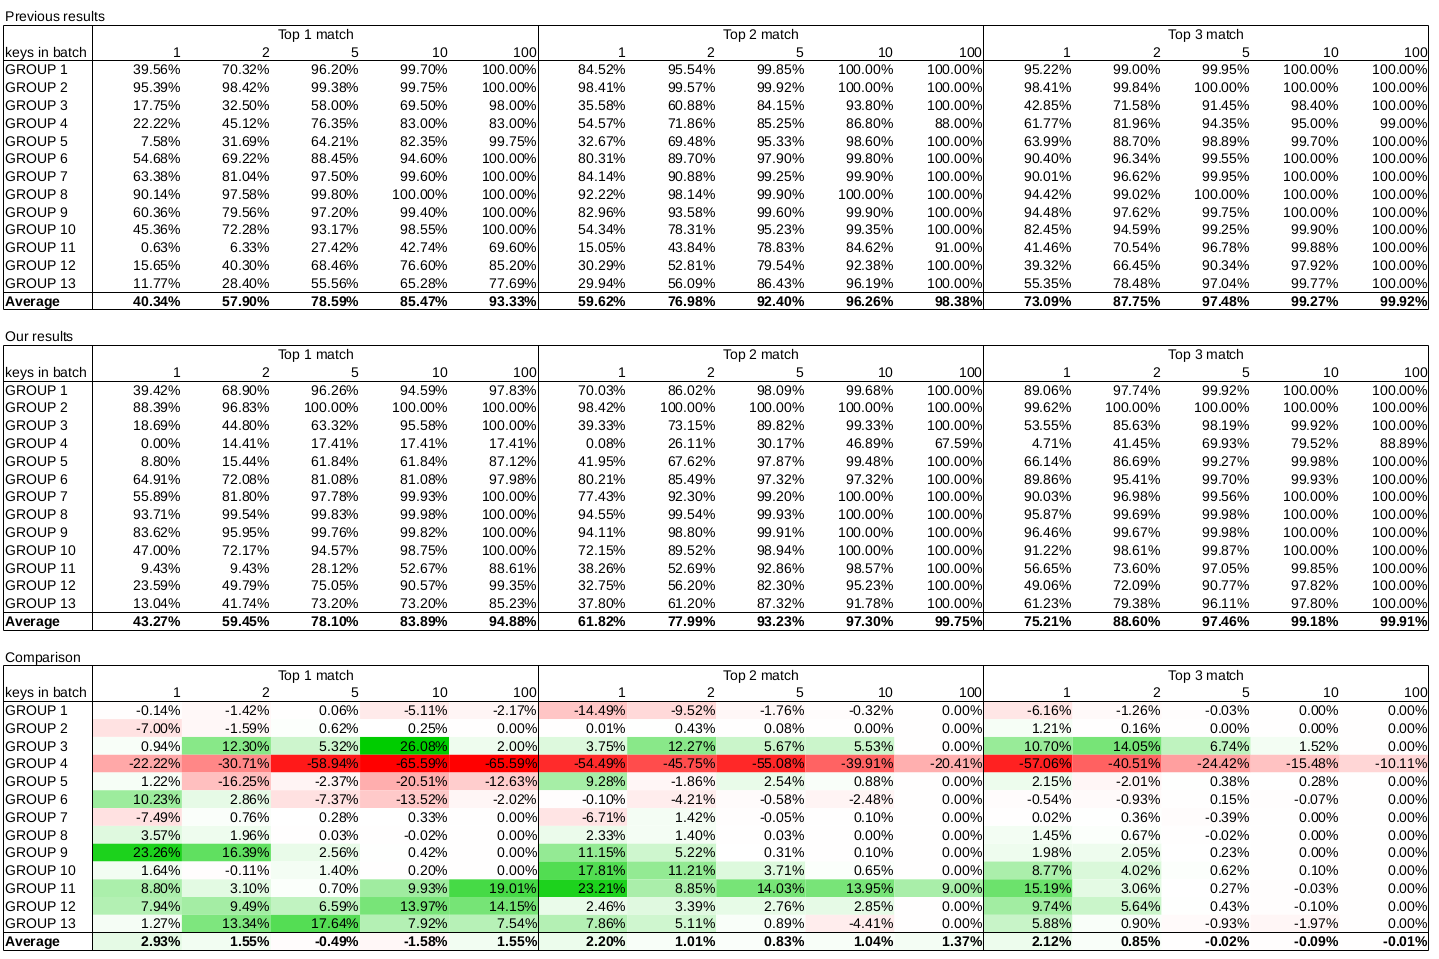
\includegraphics[width=\textwidth]{tex/images/results/comparison_13}
\caption{Comparison of results of CROCS lab and our model.}
\label{comparison-results}


\end{sidewaysfigure}


\textbf{TODO}
\begin{itemize}

\item binary classifiers
\item 64 groups

\end{itemize}

